\chapter{Stand van zaken}
\label{ch:stand-van-zaken}

\section{De wereld van de spraakgestuurde technologie}
\subsection{Spraakgestuurde technologie}
Er zijn een aantal begrippen die met het thema te maken hebben, maar die niet hetzelfde omvatten. Spraaktechnologie of taal- en spraaktechnologie is een verzamelnaam voor allerlei technieken waarmee de computer communiceert met zijn gebruiker door middel van menselijke taal.[bron6] Het is de poging van de computer om de menselijke taal na te bootsen.

Spraaktechnologie wordt vaak geassocieerd met spraakherkenning. Volgens [bron7] is spraakherkenning de kunst van de computer om gesproken taal te identificeren en om te zetten naar voor de computer leesbare machinetaal. Dit is echter maar één techniek die gebruikt wordt binnen de spraaktechnologie. Een tweede techniek, die net het omgekeerde is van spraakherkenning, is spraaksynthese. Volgens dezelfde bron is spraaksynthese menselijke spraak dat ontwikkeld wordt door een computer. Het wordt gebruikt om geschreven tekst om te zetten naar gesproken taal, geproduceerd door de computer.

Deze twee technieken zijn essentieel in het ontwikkelen van een voice user interface, ofwel stemgestuurde gebruikersomgeving, waar de gebruiker de computer als het ware bedient met zijn stem in plaats van bijvoorbeeld een toetsenbord of aanrakingen. De computer moet de gesproken taal van de gebruiker begrijpen (spraakherkenning) en moet een gepast antwoord teruggeven (spraaksynthese).

Spraaktechnologie omvat naast deze twee begrippen nog meer. Denk maar aan spelling- en grammaticacontrole, spraak- en tekstanalyse, automatische vertalingen, enzovoort.

% Nog eens goed bekijken, Verschil Voice User Interface en spraakassistenten

\subsection{De bekende spraakassistenten}
Welke talen kan het nu en in de nabije toekomst ondersteunen?
-> allemaal in eenzelfde tabel
-> Van elke spraakassistent zeggen van: ‘Volgens -naam bedrijf- is -naam spraakassistent- … De prijs is ook interessant om mee te delen.

Dit onderzoek vergelijkt twee van de meest prestigieuze spraakassistenten, namelijk Google’s Assistant en Amazon’s Alexa. Daarnaast wordt nog … MYCROFT, wat is het precies?

Slimme spraakassistenten worden alleen maar slimmer. [bron4] heeft onderzocht hoe hoog het intelligentieniveau is van 4 slimme assistenten, namelijk Google Assistant, Microsoft Cortana, Amazon Alexa en Apple Siri in 2017 en 2018. De geanalyseerde gegevens zijn de antwoorden van de assistenten op 5000 algemene vragen. De beste prestatie werd verricht door Google Assistant die op 77,2 procent van de vragen een antwoord kon bieden, waarvan 95 procent correct. Bij alle assistenten zie je een verhoging van de intelligentie in vergelijking met het vorige jaar.
\begin{figure}[h]
    \centering
    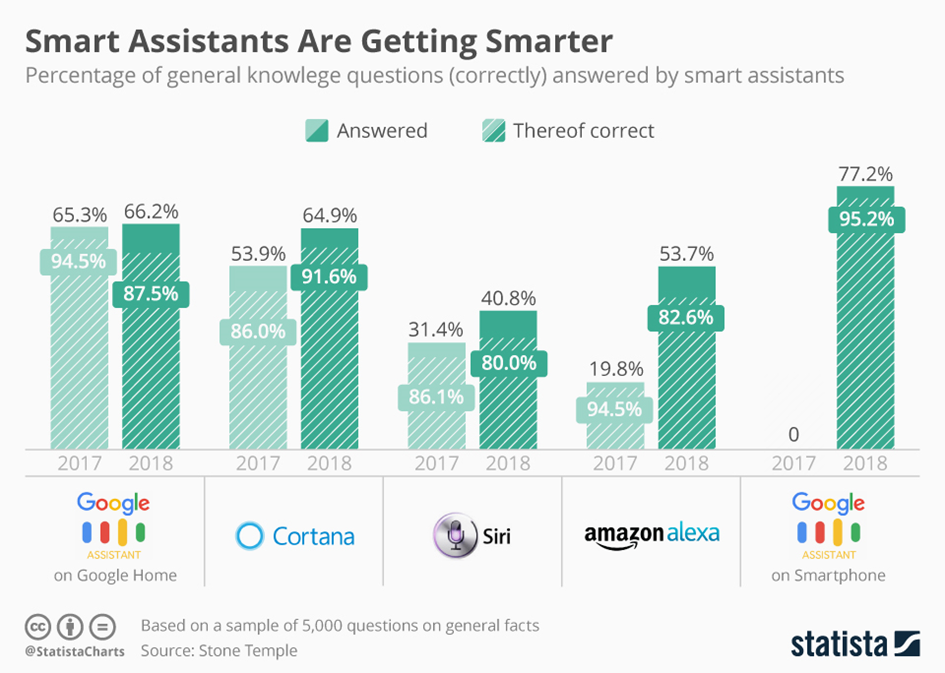
\includegraphics[width=0.7\linewidth]{img/SmartAssistantsAreGettingSmarter}
    \caption{Hoe hoog ligt het intelligentieniveau bij slimme spraakassistenten}
    \label{fig:smartassistantsaregettingsmarter}
\end{figure}

Mycroft.AI maakt gebruik van de Mimic technologie om tegen de gebruiker te praten.

\section{Eerste hulp bij ongevallen}
De AED of automatische externe defibrillator is een toestel dat een elektrische schok geeft om het hartritme te herstellen bij een hartaanval. Om verwarring te vermijden, bij een hartstilstand staat het hart niet echt stil, maar stopt het met functioneren door het gevolg van hartritmestoornissen. Defibrilleren doet het hart echter wel stilstaan, zodanig dat de normale hartmechanismen de controle opnieuw kunnen overnemen. [bron3] Volgens [bron1] heeft het belang van vroegtijdig defibrilleren voor het verhogen van de overlevingskans geleid tot het concept van de ‘eerste hulp’-defibrillatie en het AED toestel. Tegenwoordig zijn er in België AED’s voorzien op verschillende openbare plaatsen zoals sporthallen, scholen of grote bedrijven om er voor zorgen dat defibrillatie vroegtijdig kan uitgevoerd worden door niet-medisch personeel, in afwachting van de komst van getraind medisch personeel.

Onderzoeken die het nut aantonen van eerste hulp enzo.

\section{Bestaande eerste hulpapplicaties}
\subsection{De Vlaamse EHBO-app van het Rode Kruis
\lipsum[7-20]
Op 2 april ’19 kwam het Rode Kruis met het nieuws dat ze een app hebben ontwikkeld die kan helpen bij het geven van eerste hulp bij ongevallen. 80 procent van de Vlamingen weet niet wat er moet gebeuren in situaties zoals een nabije persoon die begint te stikken, een hartstilstand krijgt of hevig begint te bloeden. Uit angst om iets fouts te doen, gebeurt er dan ook vaak niks. Met de app willen ze zoveel mogelijk mensen in staat stellen om hulp te verlenen. [bron2]

Het Rode Kruis benadrukt dat de applicatie de opleiding niet kan vervangen, maar dat het hulp kan bieden bij het geven van eerste hulp.

In de applicatie zijn er twee grote onderdelen, leer eerste hulp en verleen eerste hulp. Dit maakt onmiddellijk duidelijk dat de app twee grote functionaliteiten heeft, namelijk directe instructies geven bij een ongeval en het aanleren van eerste hulp bij ongevallen. Daarnaast kan de gebruiker met behulp van de app een AED zoeken in de buurt. Er zijn ook nog enkele opties die je naar de website van het Rode Kruis brengen om informatie te verkrijgen over het geven van bloed of plasma, het doen van een gift, het volgen van een opleiding of het worden van een vrijwilliger.

Als je wilt leren over eerste hulp kan je eerst een onderwerp zoals een alcoholvergiftiging of een beroerte kiezen. Daarna krijg je over het onderwerp informatieteksten, video’s, vragen & antwoorden. Per leerdeel krijg je een vraag of een quiz die je moet oplossen om bepaalde badges te verdienen.

Als je eerste hulp wilt verlenen kan je uit het overzicht een onderwerp over eerste hulp kiezen, waarna je informatie krijgt over wat je moet vaststellen en wat heb nodig hebt. Daarnaast geeft de app ook een stappenplan van instructies wat je moet doen. De levensbedreigende situaties staan helemaal bovenaan opgelijst en zijn voorzien van extra gesproken instructies.

Het localiseren van AED toestel is pas beschikbaar op 15 april.

\subsection{De Nederlandse EHBO-app van het Rode Kruis}
Deze en andere apps vooral vergelijken met Vlaamse EHBO-app, want die staat centraal in dit onderzoek. Of gewoon veel korter beschrijven.
